\newpage
\section{Fortran 语言简介}
\subsection{编程语言与Fortran的发展}
计算机只认识机器语言,机器语言是由二进制数(0和1)组成的指令序列。

机器语言难以理解和编写,因此需要更高级的编程语言来简化编程过程。
其它语言需要经过编译器翻译成机器语言才能被计算机执行。

为了方便编写程序,发展出了汇编语言,汇编语言只是特定功能的二进制数的助记符,而汇编语言的编译器实际上更像“文本替换器”,
只是把特定字母和符号替换成机器语言指令。

随后便发展出了更高级的编程语言,如 Fortran、C、C++、Java 等,这些语言更接近人类的自然语言,
使得编程更加直观和易于理解。

Fortran是最古老的高级编程语言之一,最初设计用于科学计算和数值分析。
目前看来有些过时,但出于其对硬件的高效利用和对数值计算的优化,以及多年积累的丰富代码库,
Fortran 仍然在科学计算领域广泛使用。

早期的Fortran版本主要有Fortran 77、Fortran 90。
Fortran也在不断发展,新版本的Fortran语言增加很多功能,如动态数组等,
Fortran 2003、Fortran 2008等版本引入了面向对象编程和并行计算等新特性,
Fortran modern是对Fortran 90及其后续版本的统称。

出于稳定性以及兼容性考虑,我们课程主要使用Fortran 77,会用到一些Fortran 90的特性。
文件扩展名统一用\code{.f}(即文件名为\code{*.f}),避免出现语言版本与文件扩展名不一致的情况。

\subsection{Fortran 与打孔卡片}

Fortran语言创始的时候,计算机还没有现代计算机键盘、屏幕等输入输出设备,主要通过打孔卡片输入程序以及输出结果。

打孔卡片格式统一,共12行(0-9共10行,上面空白处2行),80列,每一列表示一个字符,每一张打孔卡片可以表示一行语句。

如
\begin{envcode}{text}{Text}
0123456789ABCDEFGHIJKLMNOPQRSTUVWXYZ,.:;'"-+=!@#$%^&*()_/<>
\end{envcode}
在打孔卡片上就如图\ref{fig:dkkp-1}显示,注意,打孔卡片不分大小写。
\begin{figure}[h]
    \centering
    \captionsetup{font={small, bf}, margin=60pt}
    \begin{subfigure}[c]{0.9\textwidth}
    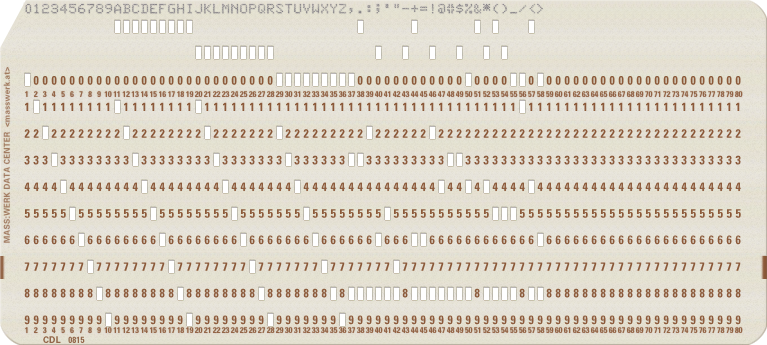
\includegraphics[width=\textwidth]{dkkp-1.png}
    \end{subfigure}    
    \caption{打孔卡片}
    \label{fig:dkkp-1}
\end{figure}

对于Fortran语言,打孔卡片的格式有一些特殊要求,称为Fortran的固定格式,每一行的要求如下:

\begin{center}

\begin{table}[!h]
        \centering
        
\begin{tabular}{|p{0.24\textwidth}|p{0.73\textwidth}|}
\hline 
 第1个字符 & 如果是字母C或*,这一行就是注释,不会被编译 \\
\hline 
 第1\textasciitilde 5个字符 & 如果是数字,就是给这一行代码取一个代号,不然只能是空格 \\
\hline 
 第6个字符 & 如果是“0”以外的任何字符,表示这一行程序接上一行 \\
\hline 
 第7\textasciitilde 72个字符 & Fortran程序代码的编写区域 \\
\hline 
 第73个字符及之后 & 保留区域,留空 \\
 \hline
\end{tabular}
        
        \end{table}
\end{center}

例如如下代码片段:
\begin{envcode}{fortran}{Fortran}
C THE FIRST FORTRAN PROGRAM
      WRITE(6,10)
   10 FORMAT(1X, 'HELLO, WORLD.')
      END
\end{envcode}
每一行在打孔卡片上就如图\ref{fig:dkkp-2}所示,每一行占一张卡片,共4张卡片。
(现在还不需要知道代码各个部分是什么意思,这里只是为了说明Fortran的固定格式和打孔卡片的概念。)

在向机器输入程序时,依次读取四张卡片即可。

\begin{figure}[h]
    \centering
    \captionsetup{font={small, bf}, margin=60pt}
    \begin{subfigure}[c]{0.48\textwidth}
      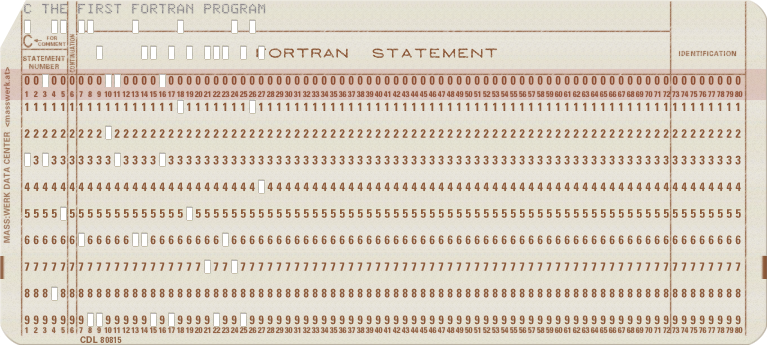
\includegraphics[width=\textwidth]{dkkp-2-1.png}
      \caption{第1行}
    \end{subfigure}
    \hfill
    \begin{subfigure}[c]{0.48\textwidth}
      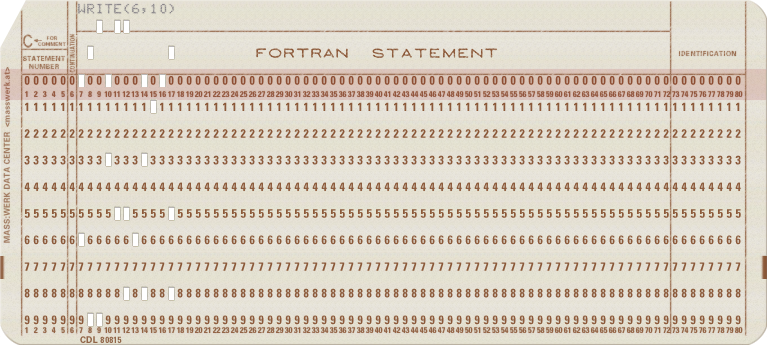
\includegraphics[width=\textwidth]{dkkp-2-2.png}
      \caption{第2行}
    \end{subfigure}
    \hfill
    \begin{subfigure}[c]{0.48\textwidth}
      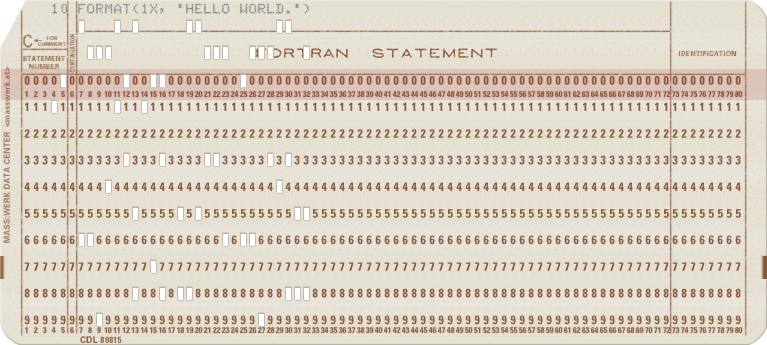
\includegraphics[width=\textwidth]{dkkp-2-3.png}
      \caption{第3行}
    \end{subfigure}
    \hfill
    \begin{subfigure}[c]{0.48\textwidth}
      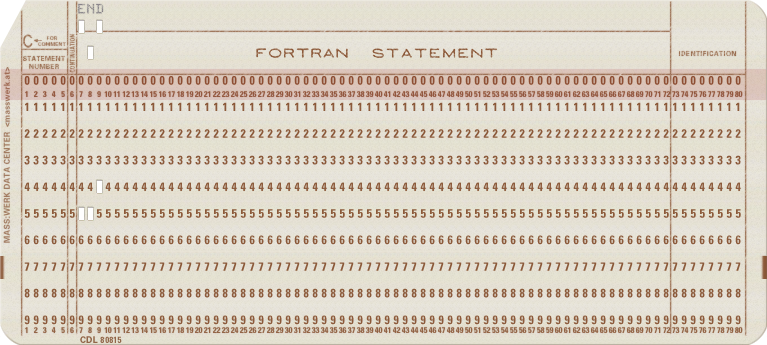
\includegraphics[width=\textwidth]{dkkp-2-4.png}
      \caption{第4行}
    \end{subfigure}    
    \caption{The first Fortran program}
    \label{fig:dkkp-2}
\end{figure}

整个程序编译后运行的输出结果为:
\begin{envcode}{text}{Text}
 HELLO, WORLD.
\end{envcode}

在打孔卡片上如图所示:
\begin{figure}[h]
    \centering
    \captionsetup{font={small, bf}, margin=60pt}
    \begin{subfigure}[c]{0.9\textwidth}
      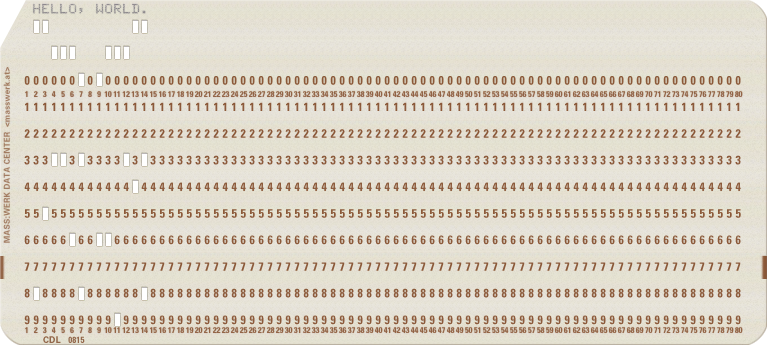
\includegraphics[width=\textwidth]{dkkp-3.png}
    \end{subfigure}    
    \caption{程序输出结果}
    \label{fig:dkkp-3}
\end{figure}

当然,现在已经没有人使用打孔卡片了,Fortran程序的编写和运行都可以在现代计算机上完成。
但是,Fortran的固定格式仍然保留了下来,Fortran程序的编写仍然需要遵循固定格式。

同时卡片的概念在Fortran中也保留了下来,
Fortran程序的每一行代码都可以看作是一张卡片,读取的每一行数据也可以看作是一张卡片。

另外,打孔卡片是不区分大小写的,Fortran程序的代码也不区分大小写。

\subsection{Fortran语言的编译}
Fortran程序需要经过编译器编译成机器语言才能被计算机执行。

在本笔记Linux部分已经提到了“gfortran”编译器的安装,如果还没有安装,可以使用以下命令安装:
\begin{envcode}{console}{Bash}
user1@host:~$ sudo apt-get install gfortran
\end{envcode}

以上面的例子为例,假设我们将代码保存在\code{learn}文件夹的\code{hello.f}:
\begin{envcode}{console}{Bash}
user1@host:~$ mkdir learn
user1@host:~$ cd learn
user1@host:~/learn$ vim hello.f
\end{envcode}

Vim编辑器用法不再重复,在文件中写入上面例子的代码,注意按照固定格式确认好空格数:
\begin{envcode}{fortran}{Fortran}
C THE FIRST FORTRAN PROGRAM
      WRITE(6,10)
   10 FORMAT(1X, 'HELLO, WORLD.')
      END
\end{envcode}

保存并退出编辑器后,使用以下命令编译程序:
\begin{envcode}{console}{Bash}
user1@host:~/learn$ gfortran -c hello.f
user1@host:~/learn$ gfortran -o hello hello.o
user1@host:~/learn$ ls
hello  hello.f  hello.o
\end{envcode}

第一条命令会生成一个目标文件\code{hello.o},第二条命令会将目标文件链接成可执行文件\code{hello}。
运行程序使用以下命令:
\begin{envcode}{console}{Bash}
user1@host:~/learn$ ./hello
 HELLO, WORLD.
\end{envcode}

如果是像这样只有一个代码文件的简单程序,或者不想生成目标文件,可以直接使用以下命令编译并运行程序:
\begin{envcode}{console}{Bash}
user1@host:~/learn$ gfortran -o hello hello.f
user1@host:~/learn$ ./hello
 HELLO, WORLD.
\end{envcode}

这样不会生成目标文件\code{hello.o},直接生成可执行文件\code{hello}。
